\textbf{Определение.} Множество функций $F = \{f\}$, определенных на $D$, называется \textbf{равностепенно непрерывным} на $D$, если $\forall \varepsilon > 0$ $\exists \delta > 0$, такое что $\forall f \in F$ и $\forall x_1, x_2 \in D$ из неравенства $|x_2 - x_1| < \delta$ $\implies$ $|f(x_2) - f(x_1)| < \varepsilon$.\\

\noindent \textbf{Лемма (Арцела-Асколи).} Пусть функции последовательности $\{f_n\}_{n=1}^{\infty}$ равномерно ограничены и равностепенно непрерывны на $[a,b]$. Тогда из нее можно выделить подпоследовательность, равномерно сходящуюся на $[a,b]$.\\
\noindent \textbf{Доказательство.} По условию
\begin{equation*}
    M = \sup_{n \in \mathbb{N}, x \in [a,b]} |f_n(x)| < +\infty
\end{equation*}
Составим последовательность чисел
\begin{equation*}
    \varepsilon_k = \frac{M}{2^{k+1}}, \quad k \in \mathbb{N}
\end{equation*}

В силу равностепенной непрерывности последовательности, по каждому $\varepsilon_k$ можно подобрать $\delta_k$, такое что если $x_1, x_2 \in [a,b]$ и $|x_2 - x_1| < \delta_k$, то для любого $n$ будет $|f_n(x_2) - f_n(x_1)| < \varepsilon_k$.

График каждой функции $f_n$ расположен в прямоугольнике $[a,b] \times [-M, M]$. Разобьем этот прямоугольник на меньшие прямоугольники с вертикальной стороной $\varepsilon_1$ и горизонтальной стороной, не превосходящей $\delta_1$ (см. \hyperref[squares]{рисунок}).

\begin{figure}[h!]\label{squares}
    \center{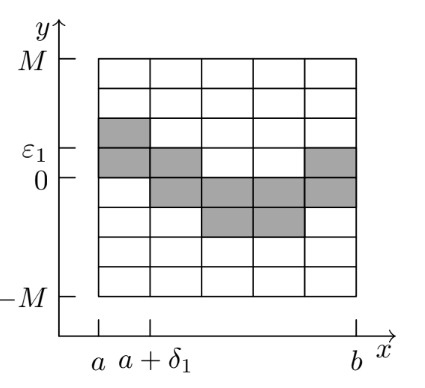
\includegraphics[scale=0.5]{Pics/Screenshot from 2021-01-14 20-32-54.png}}
\end{figure}

График каждой фукнции $f_n$ проходит не более, чем по двум соседним прямоугольникам каждой вертикальной полосы. Количество смежных пар прямоугольников в первой полосе конечно. Значит, найдется пара, по которой проходит бесконечное множество графиков функции последовательности --- закрасим ее. Будем рассматривать теперь только те функции, графики которых проходят по закрашенным прямоугольникам. Во второй полосе выберем пару соседних прямоугольников, через которые проходит бесконечное множество функций из выбранного семейства. Эту пару также закрасим и далее будем рассматривать только те функции, графики которых проходят по закрашенной области.

За конечное число шагов доберемся до крайней правой полосы. Таким образом, получим множество (закрашено на \hyperref[squares]{рисунке}), внутри которого проходят графики функций некоторой последовательности $F_1^{*} = \{f_{n_k}\}$. Для любых функций $f, g \in F_1^{*}$ верно: $|f(x) - g(x)| < 2\varepsilon_1$ при любом $x \in [a,b]$.

Выберем первую функцию из $F_1^{*}$ и обозначим ее $f_1^{*}$. Проведем те же рассуждения для оставшейся последовательности. Получим последовательность $\{f_n^{*}\}$.

По критерию Коши докажем, что последовательность $\{f_n^{*}\}$ сходится равномерно на $[a,b]$.

Зафиксируем $\varepsilon > 0$. Найдем такое $N$, что $2\varepsilon_N < \varepsilon$. При любом $k \in \mathbb{N}$ будет $f_N^*, f_{N+k}^* \in F_N^*$, поэтому при любом $x \in [a,b]$
\begin{equation*}
    |f_N^*(x) - f_{N + k}^*(x)| < 2\varepsilon_N < \varepsilon
\end{equation*}
Таким образом, последовательность $\{f_n^*\}$ сходится равномерно.
